\documentclass[conference,compsoc]{IEEEtran}

% *** CITATION PACKAGES ***
%
\ifCLASSOPTIONcompsoc
  % IEEE Computer Society needs nocompress option
  % requires cite.sty v4.0 or later (November 2003)
  \usepackage[nocompress]{cite}
\else
  % normal IEEE
  \usepackage{cite}
\fi
% cite.sty was written by Donald Arseneau
% V1.6 and later of IEEEtran pre-defines the format of the cite.sty package
% \cite{} output to follow that of the IEEE. Loading the cite package will
% result in citation numbers being automatically sorted and properly
% "compressed/ranged". e.g., [1], [9], [2], [7], [5], [6] without using
% cite.sty will become [1], [2], [5]--[7], [9] using cite.sty. cite.sty's
% \cite will automatically add leading space, if needed. Use cite.sty's
% noadjust option (cite.sty V3.8 and later) if you want to turn this off
% such as if a citation ever needs to be enclosed in parenthesis.
% cite.sty is already installed on most LaTeX systems. Be sure and use
% version 5.0 (2009-03-20) and later if using hyperref.sty.
% The latest version can be obtained at:
% http://www.ctan.org/pkg/cite
% The documentation is contained in the cite.sty file itself.
%
% Note that some packages require special options to format as the Computer
% Society requires. In particular, Computer Society  papers do not use
% compressed citation ranges as is done in typical IEEE papers
% (e.g., [1]-[4]). Instead, they list every citation separately in order
% (e.g., [1], [2], [3], [4]). To get the latter we need to load the cite
% package with the nocompress option which is supported by cite.sty v4.0
% and later.





% *** GRAPHICS RELATED PACKAGES ***
%
\ifCLASSINFOpdf
  % \usepackage[pdftex]{graphicx}
  % declare the path(s) where your graphic files are
  % \graphicspath{{../pdf/}{../jpeg/}}
  % and their extensions so you won't have to specify these with
  % every instance of \includegraphics
  % \DeclareGraphicsExtensions{.pdf,.jpeg,.png}
\else
  % or other class option (dvipsone, dvipdf, if not using dvips). graphicx
  % will default to the driver specified in the system graphics.cfg if no
  % driver is specified.
  % \usepackage[dvips]{graphicx}
  % declare the path(s) where your graphic files are
  % \graphicspath{{../eps/}}
  % and their extensions so you won't have to specify these with
  % every instance of \includegraphics
  % \DeclareGraphicsExtensions{.eps}
\fi
% graphicx was written by David Carlisle and Sebastian Rahtz. It is
% required if you want graphics, photos, etc. graphicx.sty is already
% installed on most LaTeX systems. The latest version and documentation
% can be obtained at: 
% http://www.ctan.org/pkg/graphicx
% Another good source of documentation is "Using Imported Graphics in
% LaTeX2e" by Keith Reckdahl which can be found at:
% http://www.ctan.org/pkg/epslatex
%
% latex, and pdflatex in dvi mode, support graphics in encapsulated
% postscript (.eps) format. pdflatex in pdf mode supports graphics
% in .pdf, .jpeg, .png and .mps (metapost) formats. Users should ensure
% that all non-photo figures use a vector format (.eps, .pdf, .mps) and
% not a bitmapped formats (.jpeg, .png). The IEEE frowns on bitmapped formats
% which can result in "jaggedy"/blurry rendering of lines and letters as
% well as large increases in file sizes.
%
% You can find documentation about the pdfTeX application at:
% http://www.tug.org/applications/pdftex

\usepackage{tikz}
\usetikzlibrary{graphs}


% *** MATH PACKAGES ***
%
\usepackage{amsmath}
% A popular package from the American Mathematical Society that provides
% many useful and powerful commands for dealing with mathematics.
%
% Note that the amsmath package sets \interdisplaylinepenalty to 10000
% thus preventing page breaks from occurring within multiline equations. Use:
%\interdisplaylinepenalty=2500
% after loading amsmath to restore such page breaks as IEEEtran.cls normally
% does. amsmath.sty is already installed on most LaTeX systems. The latest
% version and documentation can be obtained at:
% http://www.ctan.org/pkg/amsmath


\usepackage{booktabs}


% *** SPECIALIZED LIST PACKAGES ***
%
\usepackage{algorithm, algpseudocode, float}
\usepackage{lipsum}
\renewcommand{\algorithmicrequire}{\textbf{Input:}}
\renewcommand{\algorithmicensure}{\textbf{Output:}}
% algorithmic.sty was written by Peter Williams and Rogerio Brito.
% This package provides an algorithmic environment fo describing algorithms.
% You can use the algorithmic environment in-text or within a figure
% environment to provide for a floating algorithm. Do NOT use the algorithm
% floating environment provided by algorithm.sty (by the same authors) or
% algorithm2e.sty (by Christophe Fiorio) as the IEEE does not use dedicated
% algorithm float types and packages that provide these will not provide
% correct IEEE style captions. The latest version and documentation of
% algorithmic.sty can be obtained at:
% http://www.ctan.org/pkg/algorithms
% Also of interest may be the (relatively newer and more customizable)
% algorithmicx.sty package by Szasz Janos:
% http://www.ctan.org/pkg/algorithmicx


\makeatletter
\newenvironment{breakablealgorithm}
  {% \begin{breakablealgorithm}
   \begin{center}
     \refstepcounter{algorithm}% New algorithm
     \hrule height.8pt depth0pt \kern2pt% \@fs@pre for \@fs@ruled
     \renewcommand{\caption}[2][\relax]{% Make a new \caption
       {\raggedright\textbf{\ALG@name~\thealgorithm} ##2\par}%
       \ifx\relax##1\relax % #1 is \relax
         \addcontentsline{loa}{algorithm}{\protect\numberline{\thealgorithm}##2}%
       \else % #1 is not \relax
         \addcontentsline{loa}{algorithm}{\protect\numberline{\thealgorithm}##1}%
       \fi
       \kern2pt\hrule\kern2pt
     }
  }{% \end{breakablealgorithm}
     \kern2pt\hrule\relax% \@fs@post for \@fs@ruled
   \end{center}
  }
\makeatother

\usepackage[colorlinks, linkcolor=blue]{hyperref}


% *** ALIGNMENT PACKAGES ***
%
\usepackage{array}
% Frank Mittelbach's and David Carlisle's array.sty patches and improves
% the standard LaTeX2e array and tabular environments to provide better
% appearance and additional user controls. As the default LaTeX2e table
% generation code is lacking to the point of almost being broken with
% respect to the quality of the end results, all users are strongly
% advised to use an enhanced (at the very least that provided by array.sty)
% set of table tools. array.sty is already installed on most systems. The
% latest version and documentation can be obtained at:
% http://www.ctan.org/pkg/array


% IEEEtran contains the IEEEeqnarray family of commands that can be used to
% generate multiline equations as well as matrices, tables, etc., of high
% quality.




% *** SUBFIGURE PACKAGES ***
%\ifCLASSOPTIONcompsoc
%  \usepackage[caption=false,font=footnotesize,labelfont=sf,textfont=sf]{subfig}
%\else
%  \usepackage[caption=false,font=footnotesize]{subfig}
%\fi
% subfig.sty, written by Steven Douglas Cochran, is the modern replacement
% for subfigure.sty, the latter of which is no longer maintained and is
% incompatible with some LaTeX packages including fixltx2e. However,
% subfig.sty requires and automatically loads Axel Sommerfeldt's caption.sty
% which will override IEEEtran.cls' handling of captions and this will result
% in non-IEEE style figure/table captions. To prevent this problem, be sure
% and invoke subfig.sty's "caption=false" package option (available since
% subfig.sty version 1.3, 2005/06/28) as this is will preserve IEEEtran.cls
% handling of captions.
% Note that the Computer Society format requires a sans serif font rather
% than the serif font used in traditional IEEE formatting and thus the need
% to invoke different subfig.sty package options depending on whether
% compsoc mode has been enabled.
%
% The latest version and documentation of subfig.sty can be obtained at:
% http://www.ctan.org/pkg/subfig




% *** FLOAT PACKAGES ***
%
%\usepackage{fixltx2e}
% fixltx2e, the successor to the earlier fix2col.sty, was written by
% Frank Mittelbach and David Carlisle. This package corrects a few problems
% in the LaTeX2e kernel, the most notable of which is that in current
% LaTeX2e releases, the ordering of single and double column floats is not
% guaranteed to be preserved. Thus, an unpatched LaTeX2e can allow a
% single column figure to be placed prior to an earlier double column
% figure.
% Be aware that LaTeX2e kernels dated 2015 and later have fixltx2e.sty's
% corrections already built into the system in which case a warning will
% be issued if an attempt is made to load fixltx2e.sty as it is no longer
% needed.
% The latest version and documentation can be found at:
% http://www.ctan.org/pkg/fixltx2e


%\usepackage{stfloats}
% stfloats.sty was written by Sigitas Tolusis. This package gives LaTeX2e
% the ability to do double column floats at the bottom of the page as well
% as the top. (e.g., "\begin{figure*}[!b]" is not normally possible in
% LaTeX2e). It also provides a command:
%\fnbelowfloat
% to enable the placement of footnotes below bottom floats (the standard
% LaTeX2e kernel puts them above bottom floats). This is an invasive package
% which rewrites many portions of the LaTeX2e float routines. It may not work
% with other packages that modify the LaTeX2e float routines. The latest
% version and documentation can be obtained at:
% http://www.ctan.org/pkg/stfloats
% Do not use the stfloats baselinefloat ability as the IEEE does not allow
% \baselineskip to stretch. Authors submitting work to the IEEE should note
% that the IEEE rarely uses double column equations and that authors should try
% to avoid such use. Do not be tempted to use the cuted.sty or midfloat.sty
% packages (also by Sigitas Tolusis) as the IEEE does not format its papers in
% such ways.
% Do not attempt to use stfloats with fixltx2e as they are incompatible.
% Instead, use Morten Hogholm'a dblfloatfix which combines the features
% of both fixltx2e and stfloats:
%
% \usepackage{dblfloatfix}
% The latest version can be found at:
% http://www.ctan.org/pkg/dblfloatfix

\usepackage{epstopdf}

\usepackage{graphicx}

% *** PDF, URL AND HYPERLINK PACKAGES ***
%
\usepackage{url}
% url.sty was written by Donald Arseneau. It provides better support for
% handling and breaking URLs. url.sty is already installed on most LaTeX
% systems. The latest version and documentation can be obtained at:
% http://www.ctan.org/pkg/url
% Basically, \url{my_url_here}.




% *** Do not adjust lengths that control margins, column widths, etc. ***
% *** Do not use packages that alter fonts (such as pslatex).         ***
% There should be no need to do such things with IEEEtran.cls V1.6 and later.
% (Unless specifically asked to do so by the journal or conference you plan
% to submit to, of course. )


% correct bad hyphenation here
\hyphenation{op-tical net-works semi-conduc-tor}


\begin{document}
%
% paper title
% Titles are generally capitalized except for words such as a, an, and, as,
% at, but, by, for, in, nor, of, on, or, the, to and up, which are usually
% not capitalized unless they are the first or last word of the title.
% Linebreaks \\ can be used within to get better formatting as desired.
% Do not put math or special symbols in the title.
\title{Project 1 Reversi}


% author names and affiliations
% use a multiple column layout for up to three different
% affiliations
\author{\IEEEauthorblockN{Name:Yi Xiang  SID:11912013}
\IEEEauthorblockA{Department: Department of Computer Science and Engineering\\
Institution: Southern University of Science and Technology\\
Email: 11912013@mail.sustech.edu.cn}}


% conference papers do not typically use \thanks and this command
% is locked out in conference mode. If really needed, such as for
% the acknowledgment of grants, issue a \IEEEoverridecommandlockouts
% after \documentclass

% for over three affiliations, or if they all won't fit within the width
% of the page (and note that there is less available width in this regard for
% compsoc conferences compared to traditional conferences), use this
% alternative format:
% 
%\author{\IEEEauthorblockN{Michael Shell\IEEEauthorrefmark{1},
%Homer Simpson\IEEEauthorrefmark{2},
%James Kirk\IEEEauthorrefmark{3}, 
%Montgomery Scott\IEEEauthorrefmark{3} and
%Eldon Tyrell\IEEEauthorrefmark{4}}
%\IEEEauthorblockA{\IEEEauthorrefmark{1}School of Electrical and Computer Engineering\\
%Georgia Institute of Technology,
%Atlanta, Georgia 30332--0250\\ Email: see http://www.michaelshell.org/contact.html}
%\IEEEauthorblockA{\IEEEauthorrefmark{2}Twentieth Century Fox, Springfield, USA\\
%Email: homer@thesimpsons.com}
%\IEEEauthorblockA{\IEEEauthorrefmark{3}Starfleet Academy, San Francisco, California 96678-2391\\
%Telephone: (800) 555--1212, Fax: (888) 555--1212}
%\IEEEauthorblockA{\IEEEauthorrefmark{4}Tyrell Inc., 123 Replicant Street, Los Angeles, California 90210--4321}}




% use for special paper notices
%\IEEEspecialpapernotice{(Invited Paper)}




% make the title area
\maketitle
\tableofcontents
% As a general rule, do not put math, special symbols or citations
% in the abstract
%\begin{abstract}

%\end{abstract}

% no keywords


% For peer review papers, you can put extra information on the cover
% page as needed:
% \ifCLASSOPTIONpeerreview
% \begin{center} \bfseries EDICS Category: 3-BBND \end{center}
% \fi
%
% For peerreview papers, this IEEEtran command inserts a page break and
% creates the second title. It will be ignored for other modes.
\IEEEpeerreviewmaketitle

\section{Preliminaries}

\subsection{Hardware \& Software}
This project is written in \emph{Python} with editor \emph{Pycharm}. The main testing platform is \emph{Windows 10 Home Edition} (version 20H2) with Intel(R) Core(TM) i5-8300H CPU @ 2.30GHz 2.30 GHz of 4 cores and 8 threads, the memory is 16GB. And the develop platform is \emph{Ubuntu 16.04.6 LTS (GNU/Linux 4.4.0-151-generic x86\_64)} with Intel(R) Xeon(R) Gold 6278C CPU @ 2.60GHz with 8 cores and 16 threads, the memory is 16GB.

Both of the \emph{python} version are 3.8.8 and the \emph{numpy} module's version is 1.20.1 .

\subsection{Problem Description}
Reversi is a \textbf{two-person zero-sum information-symmetry} board game. Two players alternate on an 8-by-8 board until there are no more pieces left to play. The rules are very simple. At first, two pieces from each side are placed alternately in the center of the board, shown as \ref{Fig1}. A player can then only place a piece in a valid position, which is defined as a piece in a valid position where there are and only opposing pieces on the line with at least one of their own pieces in eight directions. At this time, will be two own pieces sandwiched by the other side of the piece flipped (into their own pieces). Neither side can choose not to do anything (in other words, each player must do something if they can do something). Unlike traditional reversi-chess, the condition for winning the game is to end the game with fewer pieces on your side than on the other side.

\begin{figure}[h]
\begin{center}
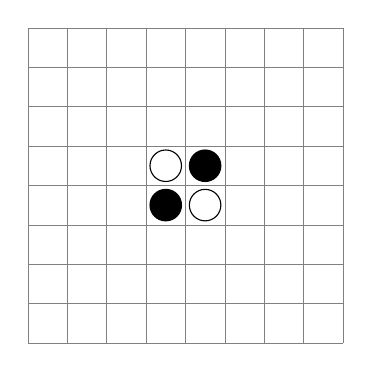
\begin{tikzpicture}[inner sep=1pt]
\draw [help lines, step=0.5] (0,0) grid (4,4);
\filldraw[fill=black] (1.75, 1.75) circle [radius=0.2];
\filldraw[fill=black] (2.25, 2.25) circle [radius=0.2];
\filldraw[fill=white] (2.25, 1.75) circle [radius=0.2];
\filldraw[fill=white] (1.75, 2.25) circle [radius=0.2];
\end{tikzpicture}
\end{center}
\caption{The initial state}
\label{Fig1}
\end{figure}

\subsection{Problem Applications}
Chess AI research focuses on game theory, or the game between two players. Such research has certain applications in urban planning and finance. In the existing studies, Yang Yuhong and Chen Zhong used evolutionary game model to describe the competition and cooperation relationship between enterprises$^{[1]}$, and Wang Yan and Dewen used evolutionary game theory to study the game process of government and enterprises in the continuous case of pollution level$^{[2]}$.

% An example of a floating figure using the graphicx package.
% Note that \label must occur AFTER (or within) \caption.
% For figures, \caption should occur after the \includegraphics.
% Note that IEEEtran v1.7 and later has special internal code that
% is designed to preserve the operation of \label within \caption
% even when the captionsoff option is in effect. However, because
% of issues like this, it may be the safest practice to put all your
% \label just after \caption rather than within \caption{}.
%
% Reminder: the "draftcls" or "draftclsnofoot", not "draft", class
% option should be used if it is desired that the figures are to be
% displayed while in draft mode.
%
%\begin{figure}[!t]
%\centering
%\includegraphics[width=2.5in]{myfigure}
% where an .eps filename suffix will be assumed under latex, 
% and a .pdf suffix will be assumed for pdflatex; or what has been declared
% via \DeclareGraphicsExtensions.
%\caption{Simulation results for the network.}
%\label{fig_sim}
%\end{figure}

% Note that the IEEE typically puts floats only at the top, even when this
% results in a large percentage of a column being occupied by floats.


% An example of a double column floating figure using two subfigures.
% (The subfig.sty package must be loaded for this to work.)
% The subfigure \label commands are set within each subfloat command,
% and the \label for the overall figure must come after \caption.
% \hfil is used as a separator to get equal spacing.
% Watch out that the combined width of all the subfigures on a 
% line do not exceed the text width or a line break will occur.
%
%\begin{figure*}[!t]
%\centering
%\subfloat[Case I]{\includegraphics[width=2.5in]{box}%
%\label{fig_first_case}}
%\hfil
%\subfloat[Case II]{\includegraphics[width=2.5in]{box}%
%\label{fig_second_case}}
%\caption{Simulation results for the network.}
%\label{fig_sim}
%\end{figure*}
%
% Note that often IEEE papers with subfigures do not employ subfigure
% captions (using the optional argument to \subfloat[]), but instead will
% reference/describe all of them (a), (b), etc., within the main caption.
% Be aware that for subfig.sty to generate the (a), (b), etc., subfigure
% labels, the optional argument to \subfloat must be present. If a
% subcaption is not desired, just leave its contents blank,
% e.g., \subfloat[].


% An example of a floating table. Note that, for IEEE style tables, the
% \caption command should come BEFORE the table and, given that table
% captions serve much like titles, are usually capitalized except for words
% such as a, an, and, as, at, but, by, for, in, nor, of, on, or, the, to
% and up, which are usually not capitalized unless they are the first or
% last word of the caption. Table text will default to \footnotesize as
% the IEEE normally uses this smaller font for tables.
% The \label must come after \caption as always.
%
%\begin{table}[!t]
%% increase table row spacing, adjust to taste
%\renewcommand{\arraystretch}{1.3}
% if using array.sty, it might be a good idea to tweak the value of
% \extrarowheight as needed to properly center the text within the cells
%\caption{An Example of a Table}
%\label{table_example}
%\centering
%% Some packages, such as MDW tools, offer better commands for making tables
%% than the plain LaTeX2e tabular which is used here.
%\begin{tabular}{|c||c|}
%\hline
%One & Two\\
%\hline
%Three & Four\\
%\hline
%\end{tabular}
%\end{table}


% Note that the IEEE does not put floats in the very first column
% - or typically anywhere on the first page for that matter. Also,
% in-text middle ("here") positioning is typically not used, but it
% is allowed and encouraged for Computer Society conferences (but
% not Computer Society journals). Most IEEE journals/conferences use
% top floats exclusively. 
% Note that, LaTeX2e, unlike IEEE journals/conferences, places
% footnotes above bottom floats. This can be corrected via the
% \fnbelowfloat command of the stfloats package.

\section{Methodology}
\begin{figure}[htbp]
\begin{center}
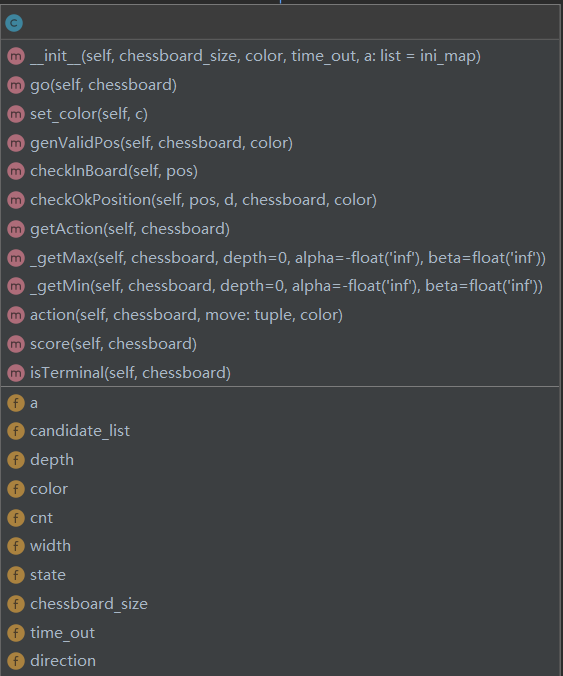
\includegraphics[width=.4\textwidth]{fig/structure.png}
\end{center}
\caption{The main structure of the project}
\label{Fig2}
\end{figure}
\subsection{Notation}
As the figure shown as above \ref{Fig2}. The main structure and the corresponding comment is shown as the table below.

% Please add the following required packages to your document preamble:
% \usepackage{booktabs}
\begin{table}[htbp]
\begin{center}
\begin{tabular}{@{}cc@{}}
\toprule
The notation                                                                          & meaning                                                                                                                                                                                      \\ \midrule
go(chessboard)                                                                        & \begin{tabular}[c]{@{}c@{}}Generate the valid moving of the AI, the \\ last position of the list is the move\\ that the AI chooses. Return nothing.\end{tabular}                             \\
\begin{tabular}[c]{@{}c@{}}genValidPos\\ (chessboard, color)\end{tabular}             & \begin{tabular}[c]{@{}c@{}}Get all the valid moving of one player, \\ the argument color determine which player\\ we choose. Return the list of moves.\end{tabular}                          \\
checkInBoard(pos)                                                                     & \begin{tabular}[c]{@{}c@{}}Check the whether the position pos\\ is in the chessboard. Return a boolean.\end{tabular}                                                                         \\
\begin{tabular}[c]{@{}c@{}}checkOkPosition\\ (pos, d, chessboard, color)\end{tabular} & \begin{tabular}[c]{@{}c@{}}Check whether the postion is ok to \\ put down a chess. The argument d is a \\ vector where the direction that is being \\ judged. Return a boolean.\end{tabular} \\
getAction(chessboard)                                                                 & \begin{tabular}[c]{@{}c@{}}Get the best move of the AI, always come\\ up with \_getMax() and \_getMin(). Return\\ a tuple, as the move.\end{tabular}                                         \\
\begin{tabular}[c]{@{}c@{}}\_getMax(chessboard,\\  depth, alpha, beta)\end{tabular}   & \begin{tabular}[c]{@{}c@{}}Get the max value and the corresponding move\\ of the AI, return a float value and a tuple.\end{tabular}                                                          \\
\begin{tabular}[c]{@{}c@{}}\_getMin(chessboard,\\  depth, alpha, beta)\end{tabular}   & \begin{tabular}[c]{@{}c@{}}Get the max value and the corresponding move\\ of the opponent, return a float value and a \\ tuple.\end{tabular}                                                 \\
\begin{tabular}[c]{@{}c@{}}action\\ (chessboard, move, color)\end{tabular}            & \begin{tabular}[c]{@{}c@{}}Generate a possible move and act it. \\ Return a temp chessboard with the origin \\ board act the move move with color.\end{tabular}                              \\
score(chessboard)                                                                     & \begin{tabular}[c]{@{}c@{}}Get the score of the chessboard. Return\\ a float value.\end{tabular}                                                                                             \\
isTerminal(chessboard)                                                                & Check if the game is end. Return a boolean.                                                                                                                                                  \\ \bottomrule
\end{tabular}
\caption{The Notation of the project}
\label{Tab1}
\end{center}
\end{table}

\subsection{Date Structure}
There are not many complex data structures are applied. The \emph{candidate\_list} is a list of the positions which have found. The \emph{MyMap} is a 2-dim matrix which specfic the value of each block of the chessboard. The \emph{chessboard} is a 2-dim matrix which specfic the game state of that time. The \emph{direction} is a list of tuple of the valid direction (the 8 directions of the connecting sides), which is used to action one move in the chessboard and obtaion the valid possible move.

\subsection{Model Design}
Firstly, I use \textbf{Brute Force} to find out all valid position for the agent to go, and successly pass the first state of the battle. I append them all to the candidate\_list.

\begin{breakablealgorithm}
\caption{The algorithm to find the valid position to go.}
\label{alg1}
\begin{algorithmic}[1]
\Require The current game-state: \emph{chessboard}
\Ensure The valid position for the agent to go
\State $idx \gets $the places that the chessboard is empty
\State $result \gets []$ 
\Comment Initial an empty list
\For {each pos in idx}
	\For {each direction in directions}
		\If {The player can flip the oppsite chess in such position and such position}
			\State append the pos in the result list
			\State break
		\EndIf
	\EndFor
\EndFor
\State\Return result
\end{algorithmic}

\end{breakablealgorithm}

Mainly, I use the alpha-beta pruning algorithm to obtain the best possible move of the agenet. For the method of getting the value of each game-states, I use the standard \textbf{multipy} in the package numpy to construct a checkerboard situation and evaluate the dot product of the matrix. 

\begin{breakablealgorithm}
\caption{The algorithm to get best move of the agent.}
\label{alg2}
\begin{algorithmic}[1]
\Require The current game-state: \emph{chessboard}
\Ensure The best move of the agent
\Function {getAction}{}
	\State $game state \gets generateState(loopCnt)$ 
	\Comment Get the game state
	\State bestValue, bestAction = getMax(chessboard, depth=0)
	\State\Return bestAction

	\Function {getMax}{chessboard, depth, $\alpha$, $\beta$}
		\If{depth==end or chessboard is terminal state}
			\State\Return score(chessboard)
			\Comment Return the score of the leaves node of the searching tree.
		\EndIf
		\State $value \gets -\inf$
		\For {each act in action\_list}
			\State new\_value $\gets getMin(action(chessboard, act)), depth+1, \alpha, \beta)$ 
			\State $value \gets max(value, new\_value)$
			\If {$\alpha \ge \beta$}
				\State break \Comment{$\beta$ cut-off}
			\EndIf
			\State\Return value, act
		\EndFor
	\EndFunction

	\Function {getMin}{chessboard, depth, $\alpha$, $\beta$}
		\If{depth==end or chessboard is terminal state}
			\State\Return score(chessboard)
			\Comment Return the score of the leaves node of the searching tree.
		\EndIf
		\State $value \gets \inf$
		\For {each act in action\_list}
			\State new\_value $\gets getMax(action(chessboard, act)), depth+1, \alpha, \beta)$ 
			\State $value \gets min(value, new\_value)$
			\If {$\alpha \le \alpha$}
				\State break \Comment{$\alpha$ cut-off}
			\EndIf
			\State\Return value, act
		\EndFor
	\EndFunction
\EndFunction
\end{algorithmic}
\end{breakablealgorithm}

\subsection{Detail of Algorithm}
For more detail of the searching algorithm, I use a \textbf{heuristic algorithm} to simply the problem. This following code will be append to the \ref{alg2} at line 9 and line 24. The algorithm is to pretreatment the action\_list and find the first \textbf{width} action to make the time usage less.

\begin{breakablealgorithm}
\begin{algorithmic}[1]
\Require{The candidate\_list}
\Ensure{The intensified candidate\_list}
\State enhance each action of the \emph{scoring function}
\State sort the list with the key score in decreasing order
\State\Return The shortlisted candidate\_list
\Comment {The shortlisted candidate\_list's length is \textbf{width}}
\end{algorithmic}
\end{breakablealgorithm}

Following, I use genetic algorithm to obtain evaluation matrix. The origin of the initial population is a combination of my subjective will and the chess score in the course reference materials. It took me quite a bit of time because we won in the opposite way to the traditional Othello.

From the first generation of fathers and mothers, we get the first generation of children. These children will have some random variation (since the original parents are identical, crossover makes no sense). We then loaded the children's scores into the AI's evaluation matrix and polled them with the same algorithm. Due to machine limitations, a large number of polls in a single round can consume a lot of time. Considering that each move takes up to five seconds, each side uses about 120 moves in total, which means that the maximum length of a single game is about 10 minutes. In the case of 100 offspring, a single round of genetic polling will consume about $C_{100}^2\times 10/24/60 \approx 34.375$ days. Counting the time spent iterating and maintaining the checkerboard, such inheritance doesn't make sense. Therefore, I adopted the method of reducing the population, and compressed the search layer number and width, and tried to get a suitable evaluation matrix in an effective time.

\begin{breakablealgorithm}
\caption{The Genetic Algorithm-From generation to generation}
\label{alg3}
\begin{algorithmic}[1]
\Require{The Parents}
\Ensure{The Childrens}
\State children $\gets$ [] \Comment{Initial the children}
\For {each child in children}
	\For {each \textbf{value} in the child score map}
		\State value $\gets$ random.choose(parents)
		\Comment {Choose randomly from mother or father.}
		\State flag $\gets$ randomInt(0, 50)
		\If {flag \% 17 == 0}
			\State value $\gets$ value + 50 - randomInt(0, 100)	
		\EndIf
		\Comment {Certain probability of variation.}
	\EndFor
\EndFor
\State\Return children
\end{algorithmic}
\end{breakablealgorithm}

In the algorithm above \ref{alg3}, I can obtain the generation from one to one randomly. Then is to get the best children in one generation. I define a module \textbf{Util.py} to create a battle system for two children to battle each other, both sides take turns at blackening. Then I statistical the winning counts of each children. Hint: there are many function I can continuing use as I have implementationed in \textbf{ai.py}.

\begin{breakablealgorithm}
\caption{The Genetic Algorithm-Battle System}
\label{alg4}
\begin{algorithmic}[1]
\Require{child A, B}
\Ensure{Result}
\State $A\gets white$
\State $B\gets black$
\State $cnt \gets 0$
\State chessboard $\gets$ initial\_board
\While {The game is not end}
	\State $cnt \gets cnt + 1$
	\If {cnt \% 2 == 0}
		\State call A.go(chessboard)
		\State move $\gets A.candidate\_list[-1]$
	\Else 
		\State call B.go(chessboard)
		\State move $\gets B.candidate\_list[-1]$
	\EndIf
	\If {move exist}
		\State action(chessboard, move)
	\EndIf
\EndWhile
\State result $\gets$ count of white and black in chessboard
\State \textbf{exchange the white and black then do the same thing}
\State\Return result
\end{algorithmic}
\end{breakablealgorithm}

After ending the wheel wars, we can get the win status of all the offspring. Then we take the first two offspring and mate with them. Get a new generation of sons for iteration. Note that I would keep the parents of this generation \emph{running} with the next generation in order to ensure that an unexpected mutation would cause the offspring to adapt to a precipitous descent. I end up with the evaluation matrix that I want.

\section{Empirical Verification}
In the process of this project, I did not submit many codes at the beginning of the second phase after the end of the first phase. In my opinion, it has the following advantages: 

\begin{itemize}
\item Avoid the influence of ranking fluctuations on their own strategies and avoid utilitarian referrals.
\item The online evaluation system sometimes leads to abnormal code test results due to network fluctuations or server abnormalities (the student assistant once mentioned problems with the server in the course group), thus causing meaningless debugging, which is very uneconomical.
\item Be responsible for own studies, artificial intelligence is just one of the major required courses, I want to be able to last the code in the form of homework at once submitted (and project grading policy is and my idea match, namely the initial stage, the score does not affect the score, only affect the score in polling).
\end{itemize}

However, there are also many disadvantages, which I have some reflections after the end of the second stage: 
\begin{itemize}
\item There is no other measure of strength other than playing chess.
\item Easy to fall into the embarrassing situation of over-fitting.
\item Online battle platform can provide log files of match information (which I learned at the end), which is a very valuable learning resource and I wasted it.
\end{itemize}  

I make up for this is that adding the previous years' \href{https://github.com/lethal233/CS303A-projects/tree/main/reversi}{code} into the battle system. It join against list but bot to join the breeding. Just as with-runners to strengthen my own code.

\subsection{Data Set}
The project is divided into two phases. In the first phase, I used the test samples provided by the platform and my own test samples to conduct preliminary tests. And after I passed the platform test, I didn't update my test sample (thinking the platform test sample was relatively complete). Shown as figure 3.

\begin{figure}[htbp]
\begin{center}
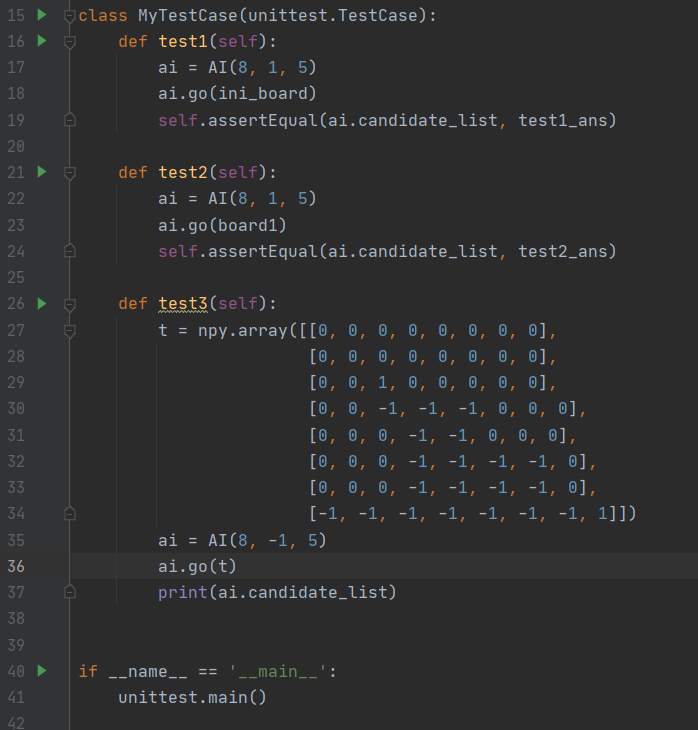
\includegraphics[width=.4\textwidth]{fig/tc.png}
\end{center}
\caption{Test cases}
\label{Fig3}
\end{figure}

In the second phase, I use the self battle system to test the strength of the agent, the evaluation criteria is the winning rate of the agents. The following section will show the winning rate with the agent and random agent.

\subsection{Performance measure}
Base on my experience of chess games, we can divide chess into early, middle and late state. The first thing we should do is to measure the number of valid positions. At this time, I use two random agents. The \textbf{random} means that they choose the position randomly, but the position they choose are always valid. Otherwise, the game cannot go on. I do such things for 100 times and get the average number of valid positions in each game, shown as the figure below.

\begin{figure}[htbp]
\begin{center}
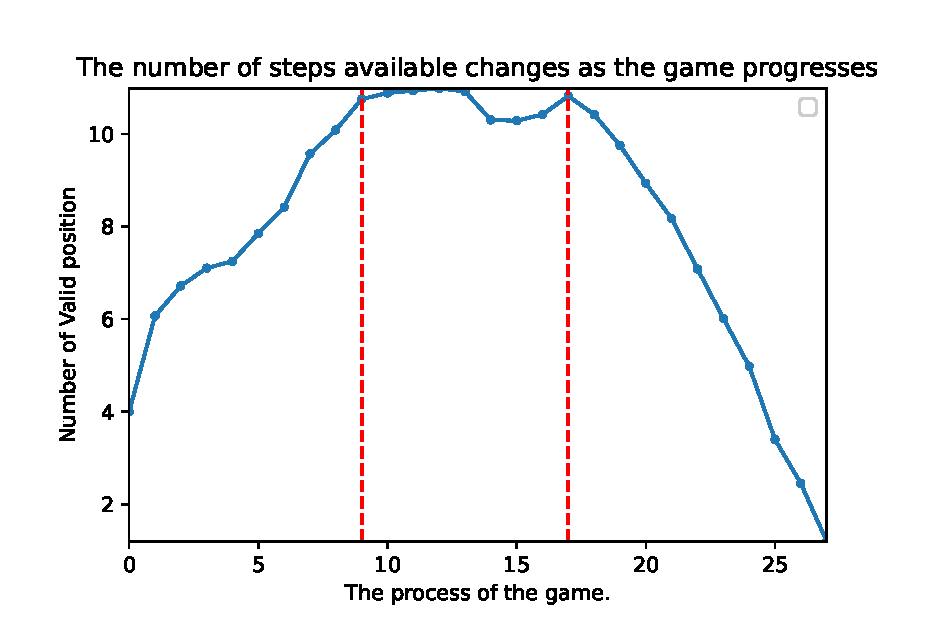
\includegraphics[width=.4\textwidth]{fig/1.eps}
\end{center}
\caption{The number of steps available changes as the game progresses}
\label{Fig4}
\end{figure}

We can obtaion the complexity of the agent search changes with the situation of game progresses. Then I define three game state for my agent. The Start game, the Middle game and the End game. The definition is shown as the following table (\textbf{cnt} means the count of steps did the game take).

\begin{table}[htbp]
\begin{center}
\begin{tabular}{@{}cc@{}}
\toprule
State       & Define           \\ \midrule
Start game  & 0$<$cnt$<$10         \\
Middle game & 10$\le$ cnt $<$20  \\
End game    & Other situations \\ \bottomrule
\end{tabular}
\end{center}
\caption{The definition of the \textbf{game state}}
\label{tab2}
\end{table}

For the three different game state, I use different ways to search the best action of the agent.

\begin{itemize}
\item [Start] In this state, since the number of valid position is not so much, I enlarge the searching width and depth, in order to maximize the value of best action.

\item [Middle] In this state, unlike the opening, I shrink the width and depth. The reason was that I could pass the local tests to limit the time, but never passed the tests after submitting the platform (it turned out to be platform load). So in order to make the submission work, I took a very conservative approach, drastically reducing the width and depth of the search in the middle of the panel to pass the basic tests. But the result is a much lower win rate.

\item [End] In this state, since the game is nearly end, and the complexity become smaller and smaller, I enlarge the searching width and depth again. More importantly, I added the judgment to check the end of the game terminal, returning a very large weight when searching for the end of a victory for your side and a very small weight when searching for the end of a victory for your opponent. This setting make sure the agent can kill the game decidedly.
\end{itemize}

From the time measuring, by doing the test of the AI self battle. I obtain the figure which show the steps for the agent cost. You may ask why I choose \textbf{28} as the totally steps. It from experience. We know that the maximum count of steps is 30. So I just choose a number smaller than it.

\begin{figure}[htbp]
\begin{center}
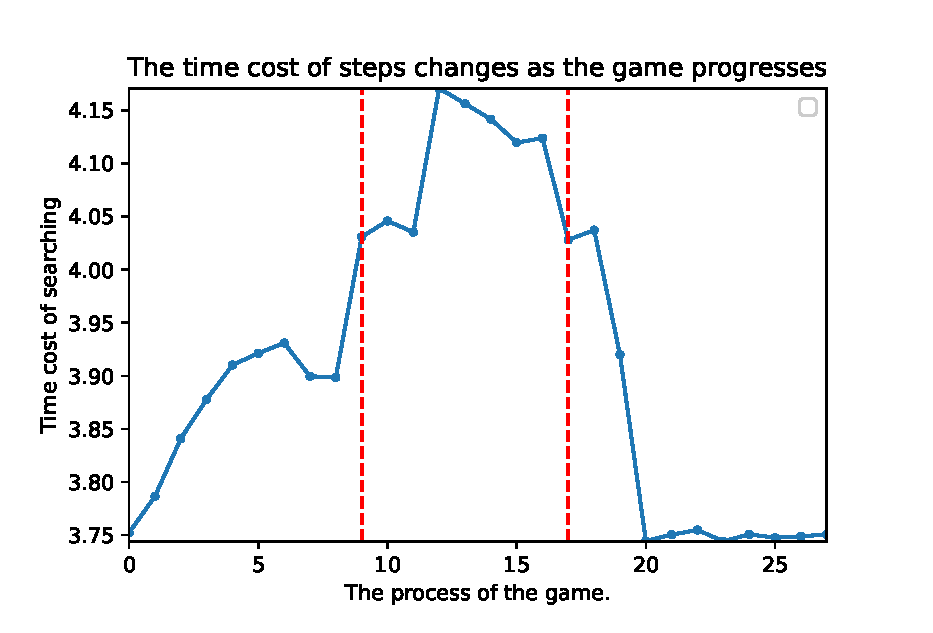
\includegraphics[width=.4\textwidth]{fig/2.eps}
\end{center}
\caption{The time cost of steps changes as the game progresses}
\label{Fig5}
\end{figure}

After dividing the situation, I am able to get a relatively reasonable time use interval locally. To make sure I passed the feasibility test, I keet it to just 4.2 seconds, which sacrificed some search accuracy, but I think it is worth it.

\subsection{Hyperparameters}
The main \textbf{Hyperparameters} of this project is the \emph{Evaluation matrix}. In this section, I will explain how I obtaion the evaluation matrix. 

Firstly, I need to initial the parent for the Genetic algorithm. Totally randomly generate it is not feasible. Because the evaluation matrix will be very ugly and useless. I got the initial evaluation matrix based on my own experience and the game with random agents. 

\begin{figure}[htbp]
\begin{center}
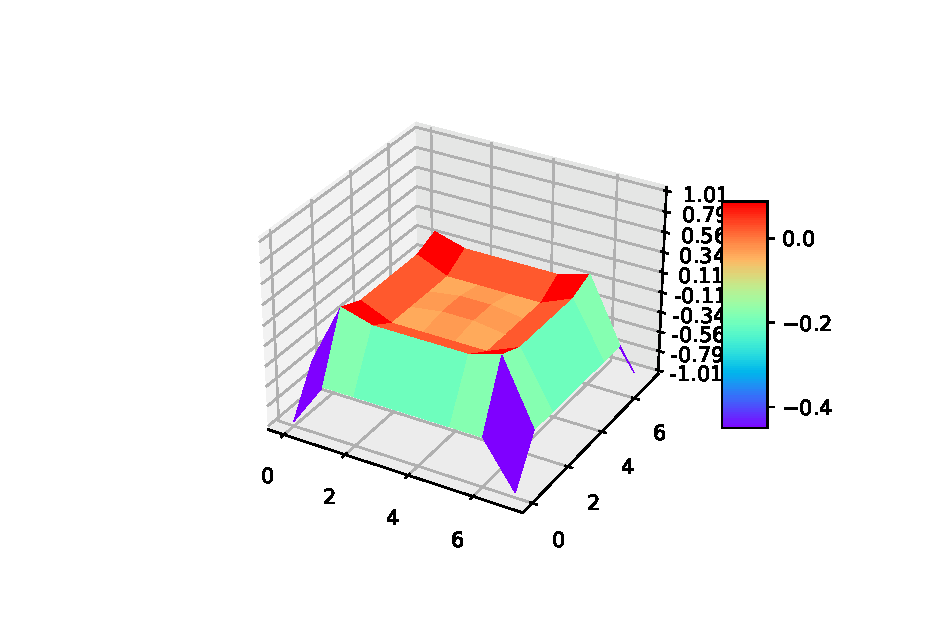
\includegraphics[width=.4\textwidth]{fig/3.eps}
\end{center}
\caption{The initial evaluation matrix}
\label{Fig6}
\end{figure}

After that I call algorithm \ref{alg3} and \ref{alg4} to evolve the generation. Due to the limitation of computation power and time, only 5 iterations were carried out. The Genetic algorithm does not converge, so the result is not very ideal. This leaves my final evaluation function almost unchanged. However, I have benefited from the experiment.

\subsection{Experimental Result}
Some of the experimenttal result is shown above like Fig.\ref{Fig4} and Fig.\ref{Fig5}. I won't go into details of them in this section.

\begin{figure}[htbp]
\begin{center}
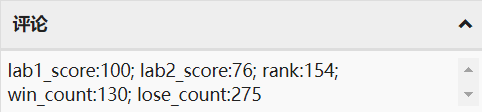
\includegraphics[width=.4\textwidth]{fig/result.png}
\end{center}
\caption{The final standing: screen-shoot from sakai}
\label{Fig7}
\end{figure}

From the comment I can get the following result. I passed all the feasibility tests in phase one, and I won 130 and failed 275 in phase two. \textbf{The winning percentage is about 32 percent} and rankings for 154. 

\subsection{Conclusion}
In general, I used alpha-beta pruning algorithm, combined with genetic algorithm to obtain a set of evaluation functions. And adopted different strategies in different stages of the game. Unfortunately, the final score was not ideal. Consider areas for improvement: 
\begin{enumerate}
\item Change the evaluation function dynamically according to the changing situation. 
\item Consider introducing the concept of stabilizers.
\item The concept of odd and even bits is introduced, which is similar to the above point, in order to reduce the occurrence of stabilizers.
\end{enumerate}

% use section* for acknowledgment
\ifCLASSOPTIONcompsoc
  % The Computer Society usually uses the plural form
  \section*{Acknowledgments}
\else
  % regular IEEE prefers the singular form
  \section*{Acknowledgment}
\fi

Thanks to the student-assistants for their wonderful questions and reliable online battle system. Thanks to Yuan Bo and Zhao Yao for their wonderful courses, thanks to Zhao Yao for his help in the LAB course.


\bibliographystyle{IEEEtran}

\begin{thebibliography}{1}
\bibitem{reference} YANG Yuhong, CHEN Zhong. Evolutionary Equilibrium Analysis on Coopetition in Intermediary Industry[J].System Engineering-Theory Methodology Applications,2006(01):26-31+38.
\bibitem{reference} WANG Yan, DING Dewen. Game analysis of public participation in environmental protection[J].Journal of Dalian Maritime University, 2006(04):19-22+35.
\end{thebibliography}





% that's all folks
\end{document}


